\documentclass[../main.tex]{subfiles}
\graphicspath{{\subfix{../images/}}, {\subfix{../diagrams/}}}

\begin{document}

    \chapter{La Pipeline di CD}
	
	    In questo capitolo descriveremo lo schema, le tecnologie e la loro applicazione per la creazione della Pipeline di \emph{Continuous Delivery}. Sarà inoltre descritto il flusso completo e dettagliato del processo stesso.
	
    	\section{Tecnologie e Strumenti}
    	
    	    \subsection{Git e Bitbucket: il \emph{trigger}}
    	    
    	        Il processo di \emph{Continuous Delivery} non viene avviato in modo automatico, la decisione spetta al team di sviluppo che, volendo effettuare una release di un determinato servizio o set di servizi, \textbf{tagga} il repository sulla \emph{master branch}. Il tag viene creato mediante \emph{Git} e segue il formato \verb|<service>/<version>|, e viene poi \emph{pushato} su \emph{BitBucket}.\\*
    	        
    	        A seguito di un nuovo \emph{tag}, BitBucket procede automaticamente a mandare un \textbf{webhook} verso \emph{Jenkins}, ovvero una richiesta contenente le informazioni salienti riguardo il tag appena creato e che verrà interpretata dal \textbf{BitBucket Plugin} installato.
    	
        	\subsection{Jenkins: il motore del processo}
        	
        	    La pipeline di \emph{Continuous Delivery} viene fatta gestire interamente da Jenkins, che si occupa di ricevere il \emph{trigger} per il suo avvio, i relativi dettagli alla compilazione da effettuare e a procedere con la compilazione stessa e l'invio degli artefatti al repository scelto. All'interno di Jenkins viene creato un oggetto di tipo \textbf{Pipeline}, che permette, mediante la scrittura di un \textbf{\emph{Jenkinsfile}}, di definire un processo sfruttando le risorse offerte dal sistema e dal linguaggio \textbf{Groovy}.\\*
        	    
        	    In particolare, la pipeline definita su Jenkins si compone delle seguenti fasi interne:
        	    \begin{enumerate}
        	        \item \textbf{Webhook Parsing}: una volta ricevuto il \emph{webhook} da parte di BitBucket, grazie al plugin dedicato, la pipeline lo parsa ed estrae il nome del servizio, la versione voluta, i target necessari alla sua compilazione e l'immagine Docker di destinazione;
        	        \item \textbf{Remote Build}: mediante l'utilizzo dell'\textbf{AWS CodeBuild Plugin}, Jenkins fa \emph{offloading} della compilazione sfruttando il servizio managed di AWS ed inviando i dettagli necessari al suo corretto funzionamento (dallo step precedente);
        	        \item \textbf{Notification}: alla fine del processo di compilazione su AWS CodeBuild, mediante il \textbf{Google Chat Plugin}, Jenkins notifica i team di sviluppo della avvenuta \emph{delivery} dell'artefatto richiesto oppure del fallimento del processo.
        	    \end{enumerate}
        	    
        	    \subsubsection{Parsing}
        	    
        	        Per effettuare il \emph{parsing} del \textbf{webhook} ricevuto da BitBucket il sistema funziona su due livelli: un \textbf{job} che sfrutta il BitBucket Plugin e che quindi può essere avviato dallo stesso, e codice \emph{Groovy} nella pipeline di delivery che effettua il parsing vero e proprio. Questa separazione è stata necessaria a causa di un bug presente nel plugin, che non permette di avviare direttamente un oggetto di tipo \emph{pipeline} su Jenkins, quindi viene avviato un \emph{job} che a sua volta avvierà la pipeline di CD.\\*
        	        
        	        In particolare, il codice nella pipeline che effettua il parsing del \emph{tag} in arrivo, sfrutta le librerie standard del linguaggio (derivate dalla JVM), ed una \emph{map} contenente i servizi abilitati alla delivery assieme ai loro dettagli:
        	        \begin{lstlisting}[language=Groovy]
def (r, t, serviceName, serviceVersion) = params.SCM_REF.split('/')

if (servicesMap.containsKey(serviceName)) {
    buildData = servicesMap[serviceName]
    buildData["version"] = serviceVersion
    buildData["scmRef"] = "refs/tags/${serviceName}/${serviceVersion}"
} else {
    currentBuild.result = 'ABORTED'
    error('The received tag contains an unsupported service')
}
        	        \end{lstlisting}
        	        
                \subsubsection{Remote Build}
        	   
        	        Per permettere a Jenkins di effettuare compilazioni remote sfruttando AWS CodeBuild si è dovuto installare il relativo plugin ufficiale fornito nel repository, assieme alla configurazione di una utenza mediante \textbf{AWS IAM} con i relativi permessi per accedere al servizio di CodeBuild. Grazie al plugin è inoltre stato possibile inserire delle variabili d'ambiente prima dell'avvio del processo di compilazione, permettendo quindi di parametrizzarlo e renderlo generico:
        	        \begin{lstlisting}[language=Groovy]
awsCodeBuild (
    credentialsType: 'jenkins',
    credentialsId: "${AWS_CREDENTIALS_ID}",
    projectName: "${CODEBUILD_SPHERE_CD_PROJECT_NAME}",
    region: "${CODEBUILD_SPHERE_CD_REGION}",
    sourceVersion: "${buildData.scmRef}",
    envVariables: "[{SERVICE, ${buildData.folder}}, {VERSION, ${buildData.version}}, {TARGET, ${buildData.target}}, {IMAGE_NAME, ${buildData.image}}]"
)
        	        \end{lstlisting}
        	
        	\subsection{AWS CodeBuild: compilazioni remote}
        	
        	    Il servizio di \emph{AWS CodeBuild} permette di creare delle pipeline per la compilazione di codice di vario genere, a partire da una definizione in formato \textbf{YAML} ed un ambiente creato mediante una immagine Docker. Per effettuare la \emph{delivery} è stato scelto l'utilizzo di CodeBuild poichè non vi è necessità di tempi di compilazione molto stretti, ne di caching durante la compilazione, quindi ogni avvio è come un \emph{fresh start} e permette di ottenere compilazioni sempre ottimizzate in tempi discreti.\\*
        	    
        	    Se per l'ambiente di compilazione viene sfruttata la stessa immagine Docker utilizzata nel processo di \emph{Continuous Integration}, la specifica di compilazione si definisce con un file \verb|buildspec.yml| nel repository che viene letto da AWS CodeBuild in fase di avvio di una build. Tale file definisce i vari step da effettuare, tra cui l'inizializzazione di Docker all'interno del container, la compilazione degli artefatti mediante \emph{Bazel}, e il caricamento degli artefatti (immagine in \verb|.tar|) in una immagine Docker finale che verrà poi pushata sul registro scelto:
        	    \begin{lstlisting}[language=Yaml]
version: 0.2

phases:
  pre_build:
    commands:
      - nohup /usr/sbin/dockerd --host=unix:///var/run/docker.sock --host=tcp://127.0.0.1:2375 --storage-driver=overlay2 &
      - timeout 15 sh -c "until docker info; do echo .; sleep 1; done"
  build:
    commands:
      - bazel build -c opt //$SERVICE:$TARGET.tar
      - docker load -i bazel-bin/$SERVICE/$TARGET.tar
  post_build:
    commands:
      - docker tag bazel/$SERVICE:$TARGET $SPHERE_REPO/$IMAGE_NAME:$VERSION
      - aws ecr get-login-password --region $SPHERE_REGION | docker login --username AWS --password-stdin $SPHERE_REPO
      - docker push $SPHERE_REPO/$IMAGE_NAME:$VERSION
        	    \end{lstlisting}
        	
        	\subsection{Docker: ambiente e artefatti}
        	\label{sec:sphere_cd_docker}
    	
    	        Nella pipeline di \emph{Continuous Delivery}, Docker viene sfruttato in due modalità differenti: per la creazione dell'ambiente di compilazione, sfruttando la \hyperref[sec:cloud_arch_docker]{stessa immagine usata nella \emph{Continuous Integration}}, sia come artefatti in output alla pipeline stessa, ovvero il prodotto che andrà poi rilasciato.\\*
    	        
    	        Ottenere immagini Docker come artefatti finali permette di sfruttare i sistemi di deployment \emph{cloud native}, come \emph{Kubernetes}, ed evitare ulteriori problemi di dipendenze essendo totalmente \emph{self contained}. Tali artefatti vengono inoltre inviati ad un \textbf{Docker Registry} in cloud, ovvero il servizio di \textbf{AWS Elastic Container Registry} (ECR), che permette di ottenere alta disponibilità online ed un sistema integrato di \textbf{Vulnerability Analysis} per ogni immagine \emph{pushata}.
    	
    	\section{Diagramma della Pipeline}
    	
    	    \begin{figure}[H]
    			\centering
    			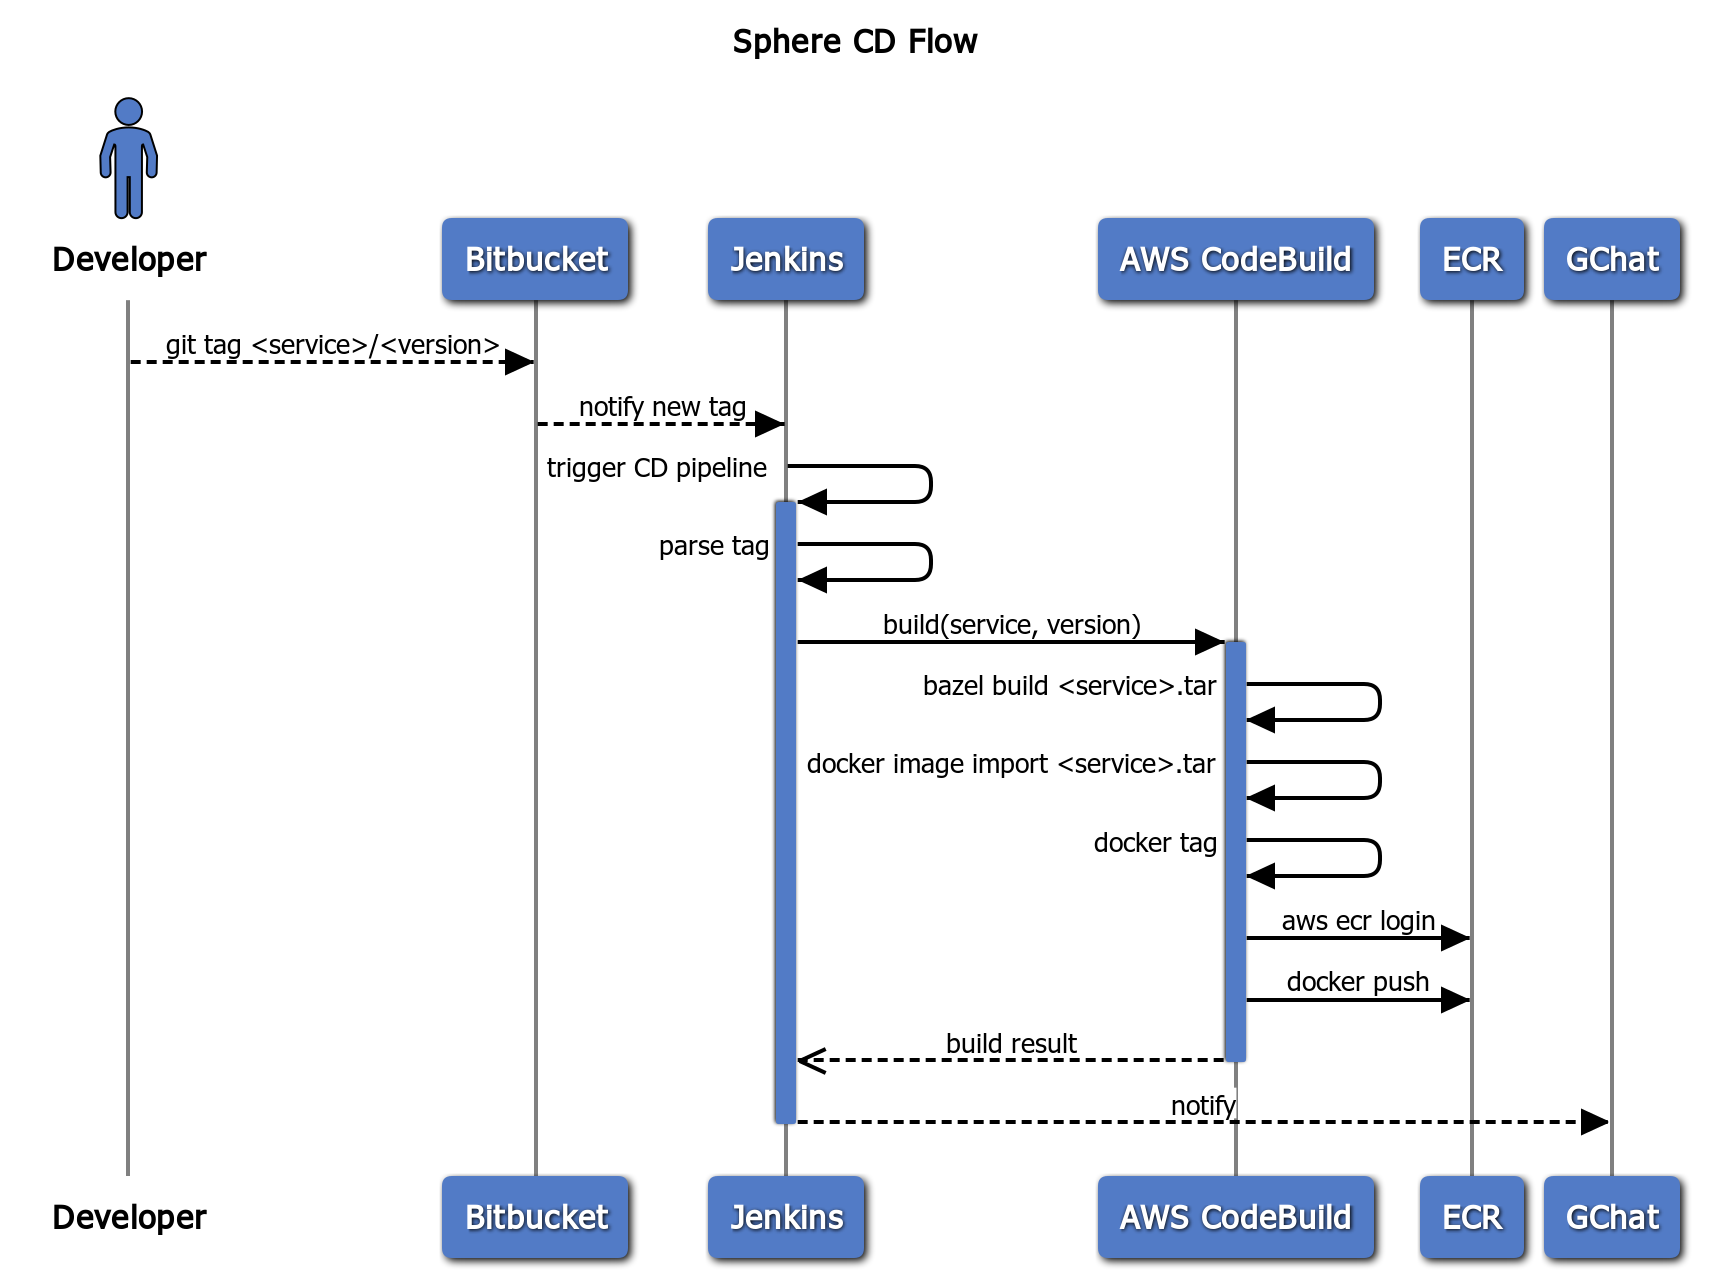
\includegraphics[width=\textwidth]{sphere_cd_flow}
    			\caption{Sphere - Continuous Delivery}
    			\label{fig:sphere_cd_flow}
    	    \end{figure}
    	
    	\section{Analisi delle Vulnerabilità}
    	
    	    Come accennato nella \hyperref[sec:sphere_cd_docker]{sezione relativa alla delivery degli artefatti}, le immagini dei servizi compilati vengono gestite da \textbf{AWS Elastic Container Registry} (ECR), un Docker Registry remoto altamente disponibile che integra una feature molto utile al fine di analisi della sicurezza dei sistemi.\\*
    	    
    	    Ad ogni \emph{push} di una nuova immagine il registry effettua una \textbf{Analisi Statica delle Vulnerabilità}, seguendo come indicazione la lista delle \textbf{Common Vulnerabilities and Exposures}\cite{cve} (CVE), ed utilizzando come strumento di analisi \textbf{Quay Clair}\cite{quay_clair}, un software \emph{open source} che permette di analizzare qualsiasi container che segua la specifica \textbf{OCI}. Nel caso in cui la gravità della vulnerabilità non sia contenuta nel repository ufficiale dei CVE, ECR utilizza il \textbf{Common Vulnerability Scoring System}\cite{cvss} (CVSS), mediante il quale computa un punteggio e lo confronta con il \textbf{National Vulnerability Database}\cite{nist_nvd} (NVD) del \textbf{NIST}.\\*
    	    
    	    Per configurare l'analisi statica delle vulnerabilità di un repository in ECR, basta abilitare tale funzione al momento della creazione dello stesso o in un secondo momento, oppure è possibile anche effettuare analisi \emph{on demand} manuali in un secondo momento.
    	
    	\section{Risultati}
    	
    	    L'introduzione di una pipeline di \emph{Continuous Delivery} ha permesso di \textbf{rimuovere} un fattore molto rilevante a livello di rilascio, ovvero la \textbf{dipendenza dal team stesso} per la compilazione e la delivery degli artefatti necessari al deployment. Precedentemente infatti il processo veniva effettuato manualmente e sulle macchine locali degli sviluppatori, che potevano impiegare diverse decine di minuti a compilare tutte le dipendenze, compilare gli artefatti software e deliverarli manualmente sul Docker Registry. Questo processo non era inoltre descritto ne documentato, rendendo ancora più difficile la delivery in casi di urgenza, dove si rendeva necessario chiedere personalmente a chi se ne fosse occupato fino a quel momento.\\*
    	    
    	    In aggiunta alla velocità e standardizzazione del processo, l'introduzione delle analisi sulle vulnerabilità ha permesso di migliorare la qualità finale degli artefatti rilasciati, rilevando ed aggiornando così eventuali dipendenze che potrebbero causare problemi di sicurezza in fase di rilascio ed utilizzo del sistema.\\*

            Riprendendo infine gli obiettivi iniziali prefissi, ed applicandoli al processo di \emph{Continuous Delivery}, possiamo stilare una tabella di conseguimento che denota il loro raggiungimento completo (con tutte le variabili del caso):
            \begin{table}[h]
    	        \centering
    	        \begin{tabular}{ |p{9cm}||p{3.5cm}|  }
                    \hline
                    \textbf{Obiettivo} & \textbf{Raggiungimento} \\
                    \hline
                    Analisi dei Requisiti per i processi CD & \cmark \\
                    Pipeline di CD per i servizi di Backend & \cmark \\
                    Infrastruttura basata su AWS per gestire il processo & \cmark \\
                    \hline
                \end{tabular}
    	        \caption{Sphere - Raggiungimento Obiettivi CD}
    	        \label{tab:sphere_obj_cd}
	        \end{table}

        \section{Esperienza Applicativa}

            Le scelte effettuate in materia di \emph{Continuous Delivery} sono state condizionate dal volere di mantenere semplice il processo, come ad esempio l'utilizzo di un servizio \emph{managed} per la compilazione come \textbf{AWS CodeBuild} al posto dello stesso sistema utilizzato nella pipeline di \emph{Continuous Integration}. Questo ha permesso di poter sviluppare un processo high level molto generico e semplice, e di poter poi modificare la fase di compilazione agendo solo sulla specifica in formato \emph{YAML} di CodeBuild, riducendo il lavoro necessario all'adattamento per altri progetti.\\*
            
            L'unico reale problema sorto durante lo sviluppo è stato causato da un bug del \textbf{BitBucket Plugin} per Jenkins, che non riusciva ad avviare con successo una pipeline configurata correttamente, poi circumnavigato grazie alla creazione di un secondo processo (Job), avviato dal plugin correttamente, che passava i dati ricevuti alla pipeline corretta.

\end{document}